% Spin-polarized DT neutron source for OpenMC -- figure summary for E. Peterson.
% Compile from spf_prototype/:  pdflatex peterson_figures.tex  (run twice)
\documentclass[11pt]{article}
\usepackage[letterpaper,margin=0.9in]{geometry}
\usepackage{graphicx}
\usepackage{amsmath}
\usepackage{float}
\usepackage[font=small,labelfont=bf]{caption}
\usepackage{microtype}
\usepackage[hidelinks]{hyperref}
\graphicspath{{figs/}}
\setlength{\parskip}{0.4em}
\pagestyle{plain}

\title{\vspace{-1.5em}Spin-Polarized DT Fusion Neutron Source in OpenMC:\\
       Verification and Blanket-Neutronics Results}
\author{}
\date{June 2026}

\begin{document}
\maketitle
\vspace{-2.5em}

\noindent
These figures summarize a self-contained prototype spin-polarized deuterium--tritium (DT)
neutron \emph{source} for OpenMC and its verification. The angular emission follows the
Schwartz (2025) differential cross section $\mathrm{d}\sigma/\mathrm{d}\Omega \propto
\tfrac34 a\,\sin^2\theta + \left(\tfrac23 b + \tfrac13 c\right)\!\left(\tfrac14 +
\tfrac34\cos^2\theta\right)$, with $\theta$ measured from the local magnetic field. The
direction sampler is verified to machine precision against a Python mirror, and the full
OpenMC transport is shown to \emph{recover} an independent analytic neutron wall load
(NWL) computed from Schwartz's closed form and his \texttt{anarr\'ima} package. The model
is then extended to scattering, a tungsten first wall, and a FLiBe breeder blanket. The
work is positioned as \emph{independent validation and a reusable tool}: it cross-validates
the Monte-Carlo spin-polarized-fuel neutronics of Bae et al.\ (\emph{Nucl.\ Fusion}
\textbf{65}, 086051, 2025) through a different source implementation (a compiled
\texttt{openmc::Source}), breeder (FLiBe vs.\ Pb-Li), and geometry. Verification figures
(1--2) use a filamentary/parabolic-ring source in a purely toroidal field with scattering
disabled; quantities are per source neutron unless noted.

\vspace{0.6em}
\noindent\footnotesize
\textbf{Scope / honesty.} The verification (Figs.~1--2) is free-streaming (no scattering),
single-energy (14.1\,MeV), with a filamentary/parabolic-ring source and a purely toroidal
field in a square (not D-shaped) cross-section. Figures~3--5 add scattering and a
single-zone FLiBe blanket (no depletion, coolant, or tritium-extraction detail; 294\,K
cross sections with 900\,K FLiBe density). No new physics is claimed: the rate/anisotropy
is Kulsrud (1982), the analytic NWL is Schwartz (2025), and Monte-Carlo SPF neutronics was
first reported by Bae et al.\ (2025). The contribution is an independently verified,
reusable OpenMC source---anchored by an analytic$\leftrightarrow$MC recovery
check---and an independent cross-validation of the published TBR-vs-polarization trend.

\clearpage

\begin{figure}[H]
  \centering
  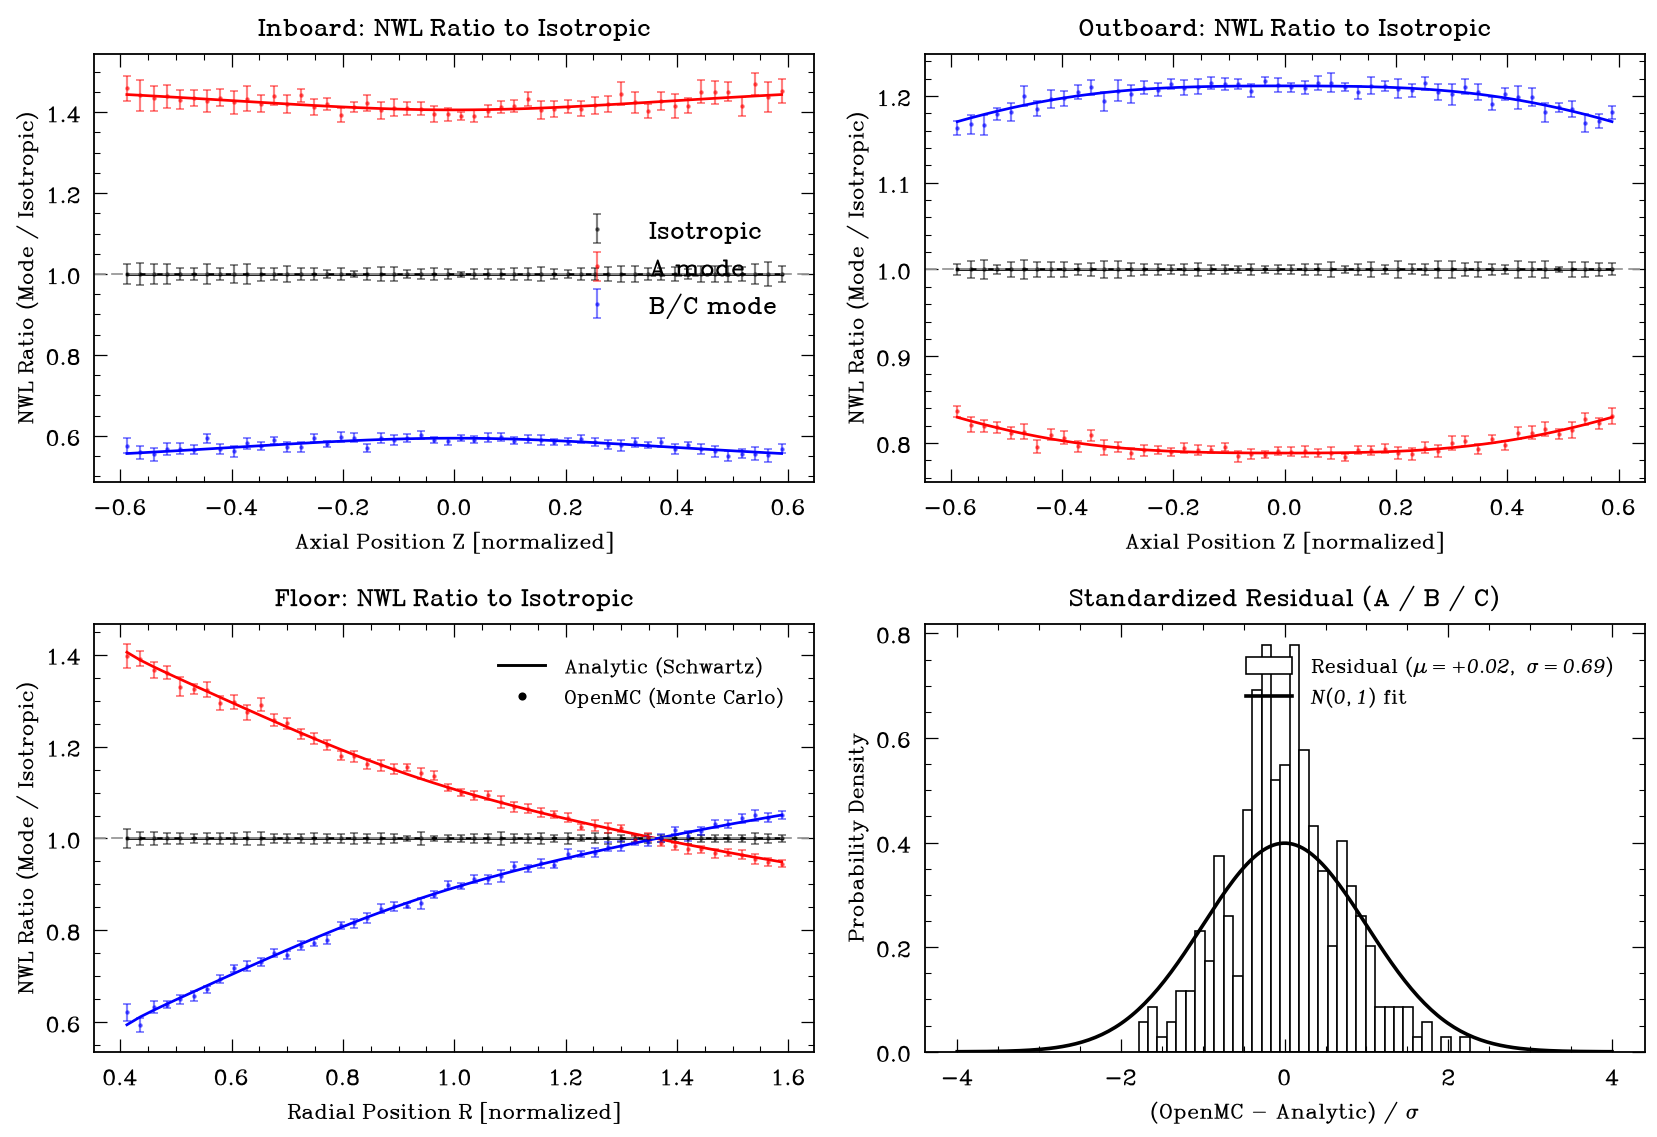
\includegraphics[width=0.95\textwidth]{tier3_analytic_vs_numerical.png}
  \caption{\textbf{OpenMC transport reproduces the analytic free-streaming NWL
  directionality.} Per-bin ratio of the neutron wall load for each pure polarization mode
  to the isotropic case, along the inboard, outboard, and floor walls of a
  square-cross-section torus (parabolic multi-ring plasma, toroidal field, scattering off).
  Markers are OpenMC Monte-Carlo transport; solid lines are the independent Schwartz
  analytic solution. The A mode ($\propto\sin^2\theta$) raises the inboard load by
  ${\sim}41\%$ and lowers the outboard by ${\sim}21\%$; the B/C mode
  ($\propto 1+3\cos^2\theta$) is the mirror image. Bottom-right: the standardized residual
  $(\mathrm{OpenMC}-\mathrm{analytic})/\sigma$ pooled over all walls and modes is
  consistent with a unit normal ($\mu=+0.02$, $\sigma=0.69$): the code reproduces the
  analytic directionality to within statistics with no detectable bias (the sub-unity
  $\sigma$ reflects mildly conservative per-bin tally errors).}
\end{figure}

\clearpage

\begin{figure}[H]
  \centering
  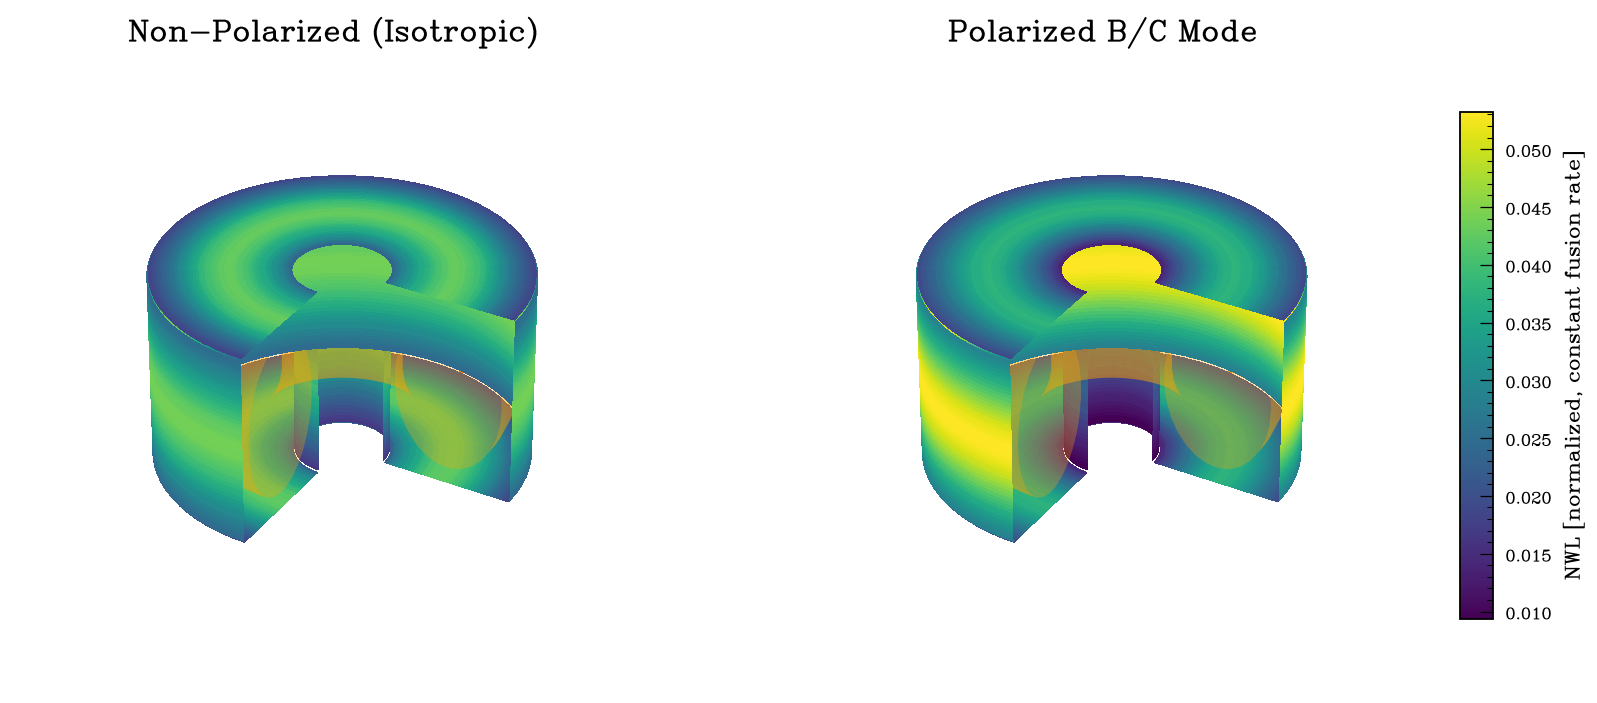
\includegraphics[width=0.93\textwidth]{tier3_torus3d.png}
  \caption{\textbf{Where the polarized source steers the wall load.} Computed
  free-streaming NWL on the four walls of the square-cross-section torus for the
  non-polarized (left) and polarized B/C (right) cases at constant total fusion rate
  (shared colour scale). This is a render of the tallied wall load, not a CAD/DAGMC
  geometry. The B/C mode steers neutrons off the inboard center stack toward the outboard
  wall---the qualitative benefit relevant to space-constrained (spherical-tokamak) center
  stacks.}
\end{figure}

\vspace{1em}

\begin{figure}[H]
  \centering
  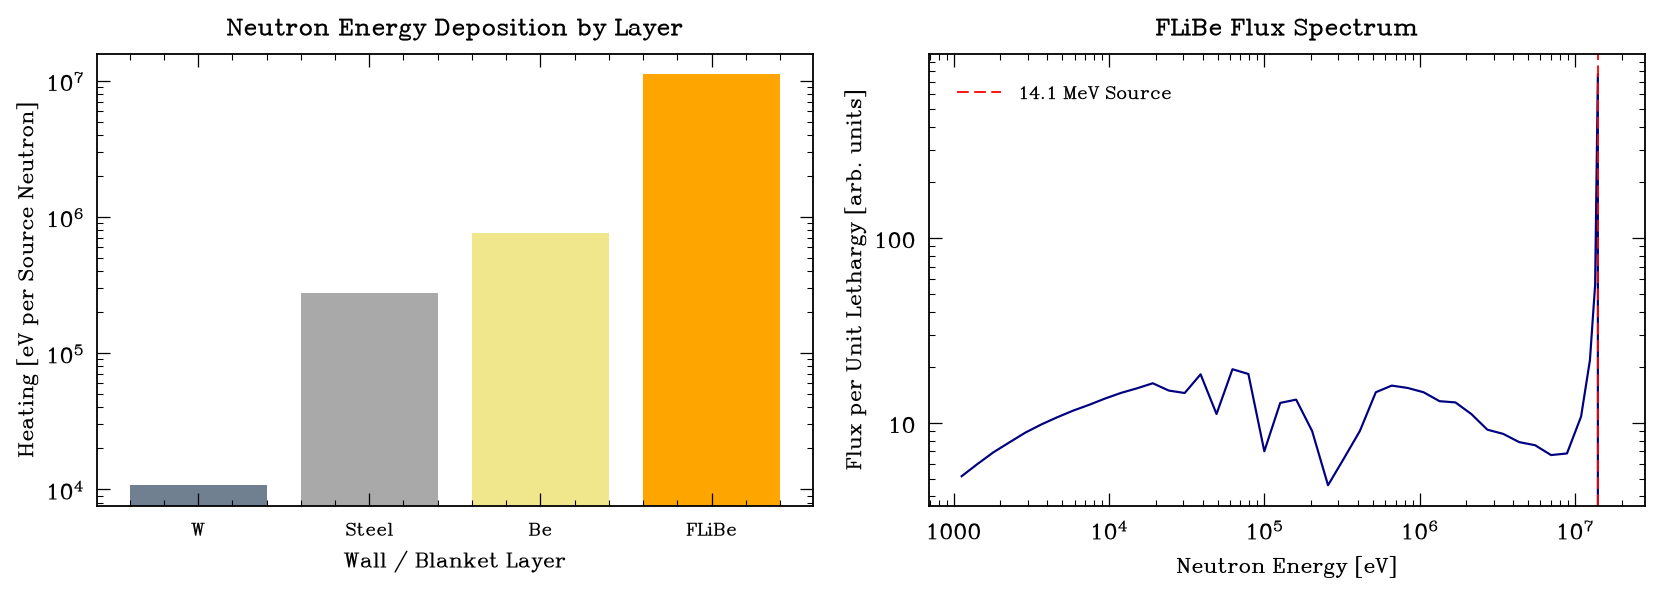
\includegraphics[width=\textwidth]{tier5_heating_spectrum.png}
  \caption{\textbf{Scattering and real materials} (cavity $\to$ W first wall $\to$ steel
  $\to$ Be multiplier $\to$ FLiBe breeder). Left: neutron energy deposition per source
  neutron by layer (log scale); the FLiBe blanket absorbs ${\sim}91\%$ of the deposited
  energy while the 1\,mm tungsten first wall takes only ${\sim}0.1\%$. Right: the FLiBe
  neutron flux spectrum, showing the 14.1\,MeV source line plus a large down-scattered
  tail to keV energies---the direct signature that scattering is active, and what drives
  low-energy $^{6}$Li breeding and material damage. Isotropic source.}
\end{figure}

\clearpage

\begin{figure}[H]
  \centering
  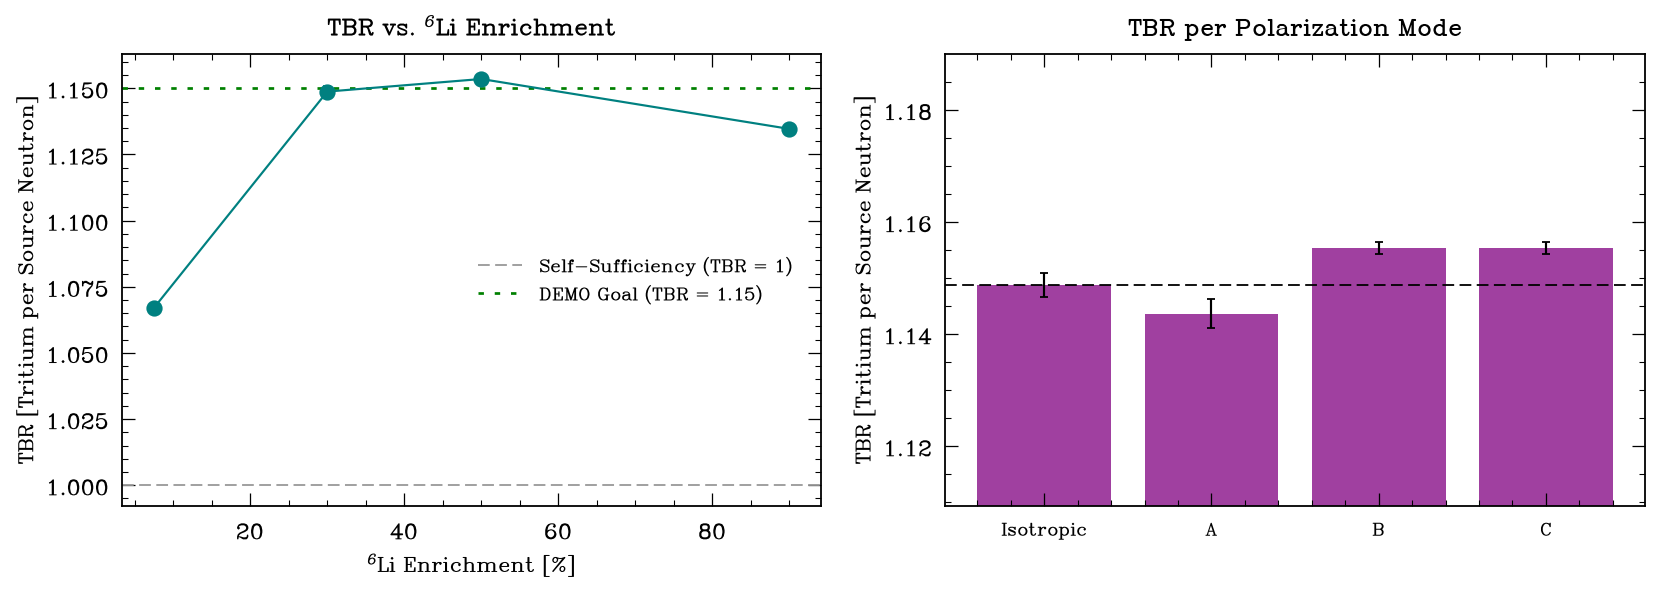
\includegraphics[width=\textwidth]{tier6_tbr.png}
  \caption{\textbf{Tritium breeding in the FLiBe blanket} (TBR $=$ tritium atoms produced
  per source neutron). Left: TBR versus $^{6}$Li enrichment (isotropic source) rises then
  plateaus near 30--50\%, reproducing the published optimum; the 30\% baseline gives
  TBR $=1.15$, in the ARC/LIBRA band at the DEMO goal. Right: TBR by polarization mode at
  constant fusion rate is only modestly polarization-dependent ($\pm0.6\%$; B/C higher,
  A lower)---the same sign as Bae et al.\ (2025) ($+2.7\%$ for parallel emission in a Pb-Li
  spherical tokamak). Steering to protect the center stack therefore costs little breeding.
  Error bars are Monte-Carlo $1\sigma$.}
\end{figure}

\vspace{1em}

\begin{figure}[H]
  \centering
  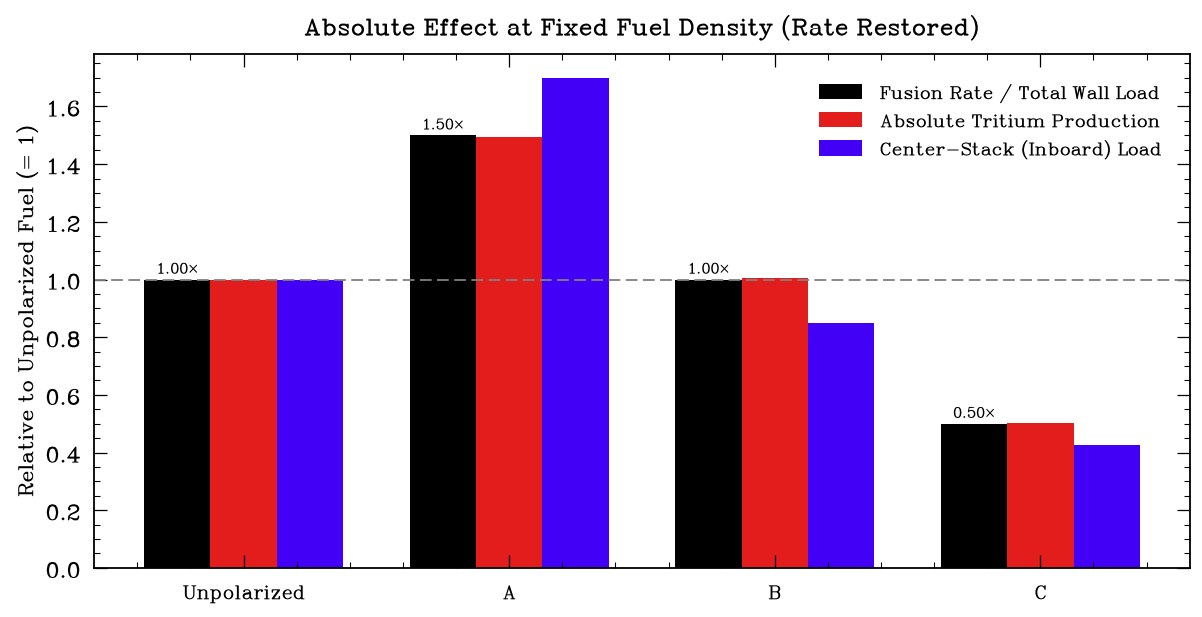
\includegraphics[width=0.78\textwidth]{tier7_absolute.png}
  \caption{\textbf{The absolute (un-normalized) effect once the reaction-rate enhancement
  is restored.} At fixed fuel density the neutron yield scales with the total-rate factor
  $\eta = a + \tfrac23 b + \tfrac13 c$, so the fully aligned A mode produces $+50\%$ more
  neutrons and the C mode $-50\%$. Bars show fusion rate, absolute tritium production, and
  absolute center-stack (inboard) load, each relative to unpolarized fuel. A is a power
  play ($+50\%$ power and tritium) but compounds the center-stack load to $1.7\times$; B
  uniquely buys directional steering ($0.85\times$ center stack) at no rate or breeding
  penalty; C halves everything. The TBR \emph{per neutron} is mode-independent, so tritium
  self-sufficiency is preserved across modes.}
\end{figure}

\end{document}
